\section{Finite Dimensional Representations of Lie Groups}
In quantum mechanics, the state space $V$ is often a $L^2$ space (like $L^2(\bR^3)$) or some subspace thereof. For a variety of reasons, we are often interested in the linear operators on $V$. In this section, we will be assuming that $V$ is finite dimensional.

\subsection{Definitions}
Let $G$ be a Lie group.
\begin{itemize}
    \item A ordinary representation of $G$ is a homomorphism $G \rightarrow GL(V)$.
    \item A projective representation of $G$ is a homomorphism $G \rightarrow PU(V)$, which we will define shortly.
\end{itemize}
When talking about ordinary representations, we often drop the word ``ordinary" and just call them representations. Observe if $G$ is a matrix Lie group, it is a representation of itself.

\subsection{}
In quantum mechanics, $V$ is also a Hilbert space, so we are often interested in unitary operators: operators that preserve the inner product. Call a representation $\Pi$ of $G$ a unitary representation if $\Pi(G) \subset U(V)$.

Recall that two vectors in the state space that differ by multiplication by a constant are considered to represent the same physical state. Thus we are also interested in the projective unitary group, which we define as
\[
    \frac{U(V)}{\{e^{i\theta}I\}} = PU(V).
\]
This is why we also study projective representations. The spaces $U(V), PU(V)$ are both Lie groups. Denote their corresponding Lie algebras as $u(v)$ and $pu(v)$.

\subsection{Irreducible Representations}
Now suppose $G$ is a compact Lie group (which will often be true in practice). Suppose we have a representation $\Pi: G \rightarrow GL(V)$. It is a theorem that if $G$ is compact and $W$ is an invariant subspace of $V$ under the operators in $\Pi(G)$, then there exists a complementary subspace $W'$ such that $W \oplus W' = V$ and $W'$ is also an invariant subspace under the operators in $\Pi(G)$. Define
\[
    \Pi'(g) = \Pi(g)|_W \in GL(W), \quad \Pi''(g) = \Pi(g)|_{W'} \in GL(W')
\]
and observe we can decompose $\Pi$ as a direct sum:
\[
    \Pi(g) = \Pi'(g) \oplus \Pi''(g) \in GL(W) \oplus GL(W') \subset GL(V).
\]
Thus we can study $\Pi$ by studying $\Pi'$ and $\Pi''$, representations of $G$ over the state subspaces $W$ and $W''$.

We call a representation $\Pi$ irreducible if the only invariant subspaces of $V$ under $\Pi(G)$ are 0 and $V$. From the discussion above, irreducible representations can be seen as building blocks of all representations of a group $G$, so it makes sense to study them in particular.

We can similarly define the notion of an irreducible projective unitary representation $\Pi: G \rightarrow PU(V)$ by considering invariant subspaces of $V$ under all $U$ such that $[U] \in \Pi(G)$.

Colloquially, if $\Pi$ is given, we sometimes say that $W$ ``is a representation of $\Pi$" if $W$ is an invariant subspace.

\subsection{Two Lemmas On De-projectivization}
Given an representation $\Sigma: G \rightarrow U(V)$, we can get a projective unitary representation $\Pi: G \rightarrow PU(V)$ by composing with the natural map $Q: U(V) \rightarrow PU(V)$. We can ask the converse: can we de-projectivize each $\Pi: G \rightarrow PU(V)$ into a map $\Sigma: G \rightarrow U(V)$? This is generally not possible. However, we can de-projectivize at the Lie algebra level:
\begin{figure}[H]
    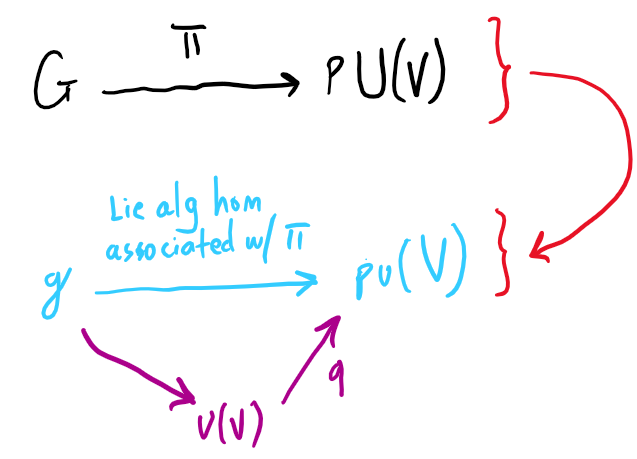
\includegraphics[width=0.5\textwidth]{figures/de-projectivization}
    \centering
\end{figure}

Here, $q: u(v) \rightarrow pu(v)$ is the Lie algebra homormorphism associated with $Q$.

We can also de-projectivize at the expense of passing from $G$ to the universal cover $G^*$.
\begin{figure}[H]
    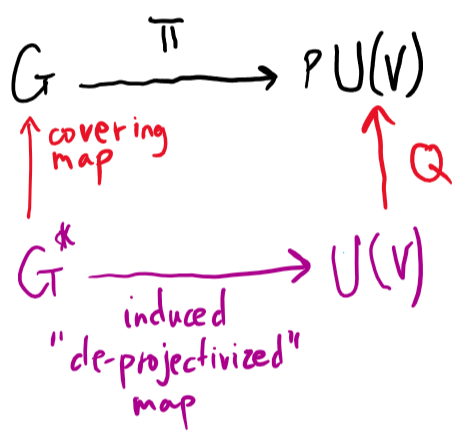
\includegraphics[width=0.4\textwidth]{figures/de-projectivization2}
    \centering
\end{figure}

\subsection{Infinite Dimensional Representations}
So far, we have only been considering the case when $V$ is finite-dimensional. We can remove this restriction if we add in extra technicial conditions in our definitions of ordinary and projective unitary representations.

However, we need worry too much about infinite dimensional representations. If $G$ is a compact Lie group, it happens that all irreducible representations of $G$ are finite-dimensional, so the representations we really have to study are finite-dimensional.
